\section{Experiments}
\label{sec:experiments}

We evaluate latent reasoning, scalability, efficiency, and representation dynamics of our shortcut-modulated looped language models. Following \cite{tay2022ul2, saunshi2025reasoning}, we compare a 24-layer, $\sim$1B-parameter non-looped Transformer with FLOP-matched looped variants. All models use a GPT-style decoder \cite{radford2019language} with NanoGPT configurations. Training is performed on a deduplicated subset of The Pile \cite{gao2020pile} for 25B tokens in accordance with Chinchilla scaling \cite{hoffmann2022training}. See \autoref{sec:supp_exp_details} for details. Unless otherwise specified, all reported results use uniform step sizes at inference: for a compute budget $M$, $\Delta_i = 1/M$ for all $i$.

\subsection{Latent Reasoning and Perplexity}
We train looped models under different parameter and compute budgets. Using the notation $(k \otimes L)$ for a $k$-block $\Phi_k$ unrolled $L$ times, we consider $k \in \{1,2,3\}$ and train with maximum loops $L \in \{8,12,24\}$. Fixed-loop models are trained and evaluated with the same $L$, whereas depth-elastic models support inference at any $M \le L$. In this section we use $kL$ as a proxy for FLOPs when comparing baselines, ignoring embedding/unembedding costs; %\hl{Supp.~X} reports throughput, memory, and the overhead of our shortcut-modulation layers.
\autoref{tab:main_table} summarizes the results for $k=3$.




\renewcommand{\arraystretch}{1.8}
\begin{table*}[t]
\centering\small
\caption{Perplexity and zero-shot reasoning for $(3\otimes 8)$ looped models under three inference budgets (24$\times$, 12$\times$, 6$\times$). At 24$\times$ we also report fixed-depth baselines; at 12$\times$/6$\times$ we compare against Base $(12\otimes 1)$ and $(6\otimes 1)$. While depth-elastic, LoopFormer narrows the perplexity gap to Base and is competitive on reasoning, outperforming other looped variants, especially at higher budgets.}

\label{tab:main_table}
\setlength{\tabcolsep}{4pt}
\fontsize{12pt}{14pt}\selectfont
\resizebox{\textwidth}{!}{%
\begin{tabular}{cccccccccccccccc}
\toprule
& \multicolumn{1}{c|}{} & \multicolumn{3}{c|}{\textbf{Perplexity} $\downarrow$} & \multicolumn{11}{c}{\textbf{Language Tasks (Accuracy)} $\uparrow$} \\
\cmidrule(lr){3-5} \cmidrule(lr){6-16}
\multirow{-2}{*}{} & \multicolumn{1}{c|}{\multirow{-2}{*}{\textbf{Params / FLOPs}}} & \textbf{Pile} & \textbf{FineWeb-Edu} & \multicolumn{1}{c|}{\textbf{OpenWebText}} & \textbf{COPA} & \textbf{HS} & \textbf{LB} & \textbf{OBQA} & \textbf{PIQA} & \textbf{Race} & \textbf{SciQ} & \textbf{ARC} & \textbf{SIQA} & \multicolumn{1}{c|}{\textbf{WG}} & \textbf{Avg Acc} \\
\midrule
\rowcolor[HTML]{F5F5F5}
\multicolumn{16}{l}{\textbf{Budget: 24x}} \\
\midrule

\multicolumn{1}{c|}{Base $(24 \otimes 1)$} &
  \multicolumn{1}{c|}{24x / 24x} &
  \textbf{9.49} &
  \textbf{20.7} &
  \multicolumn{1}{c|}{\textbf{20.08}} &
  61 &
  \textbf{35.04} &
  \textbf{41.96} &
  27.6 &
  \textbf{66} &
  29 &
  \textbf{70.1} &
  \textbf{33.43} &
  {\ul 38.18} &
  \multicolumn{1}{c|}{50.4} &
  45.27 \\
\multicolumn{1}{c|}{Base-Loop $(3 \otimes 8)$} &
  \multicolumn{1}{c|}{3x / 24x} &
  10.91 &
  24.53 &
  \multicolumn{1}{c|}{24.53} &
  61 &
  30.46 &
  34.68 &
  27 &
  63.22 &
  28.8 &
  63.7 &
  31.71 &
  \textbf{38.43} &
  \multicolumn{1}{c|}{49.8} &
  42.88 \\
\multicolumn{1}{c|}{TMLT  $(3 \otimes 8)$} &
  \multicolumn{1}{c|}{3x / 24x} &
  10.38 &
  {\ul 22.87} &
  \multicolumn{1}{c|}{21.99} &
  65 &
  {\ul 32.34} &
  {\ul 39.06} &
  {\ul 27.8} &
  63.11 &
  {\ul 29.67} &
  {\ul 69.8} &
  31.67 &
  36.95 &
  \multicolumn{1}{c|}{51.54} &
  44.69 \\ \hline
\multicolumn{1}{c|}{Naive-Loop-EE $(3 \otimes 8)$} &
  \multicolumn{1}{c|}{3x / 24x} &
  11.6 &
  26.55 &
  \multicolumn{1}{c|}{25.64} &
  \textbf{66} &
  29.68 &
  31.52 &
  27 &
  62.24 &
  28.33 &
  65.5 &
  31.64 &
  36.64 &
  \multicolumn{1}{c|}{50.59} &
  42.91 \\
\multicolumn{1}{c|}{Base-Loop-EE-Cons $(3 \otimes 8)$} &
  \multicolumn{1}{c|}{3x / 24x} &
  11.56 &
  25.33 &
  \multicolumn{1}{c|}{24.41} &
  \textbf{66} &
  30.54 &
  32.19 &
  26.8 &
  62.13 &
  28.23 &
  64.9 &
  31.45 &
  37.4 &
  \multicolumn{1}{c|}{\textbf{52.88}} &
  43.25 \\
\multicolumn{1}{c|}{TMLT-EE $(3 \otimes 8)$} &
  \multicolumn{1}{c|}{3x / 24x} &
  10.7 &
  24.07 &
  \multicolumn{1}{c|}{23.17} &
  65 &
  31.03 &
  35.14 &
  \textbf{28.4} &
  63.11 &
  28.8 &
  68.8 &
  31.74 &
  37.41 &
  \multicolumn{1}{c|}{50.83} &
  44.03 \\
\rowcolor[HTML]{DDEEFF} 
\multicolumn{1}{c|}{LoopFormer - Ours $(3 \otimes 8)$} &
  \multicolumn{1}{c|}{3x / 24x} &
  {\ul 10.28} &
  {\ul 22.87} &
  \multicolumn{1}{c|}{{\ul 21.98}} &
  \textbf{66} &
  32.3 &
  38.27 &
  26.8 &
  {\ul 63.33} &
  \textbf{30.81} &
  68 &
  {\ul 32.71} &
  37.97 &
  \multicolumn{1}{c|}{{\ul 51.94}} &
  44.81 \\ \hline
\rowcolor[HTML]{F5F5F5} 


\midrule
\rowcolor[HTML]{F5F5F5}
\multicolumn{16}{l}{\textbf{Budget: 12x}} \\
\midrule

\multicolumn{1}{c|}{Base (12x1)} &
  \multicolumn{1}{c|}{12x / 12x} &
  \textbf{9.98} &
  \textbf{22.24} &
  \multicolumn{1}{c|}{\textbf{ 21.41}} &
  {\ul 67} &
  \textbf{32.72} &
  \textbf{37.78} &
  26.2 &
  \textbf{64.69} &
  \textbf{29.86} &
  \textbf{69.1} &
  \textbf{32.29} &
  \textbf{38.38} &
  \multicolumn{1}{c|}{{\ul 51.3}} &
  44.93 \\
\multicolumn{1}{c|}{Naive-Loop-EE $(3 \otimes 4)$} &
  \multicolumn{1}{c|}{3x / 12x} &
  11.66 &
  26.74 &
  \multicolumn{1}{c|}{25.81} &
  65 &
  29.35 &
  31.28 &
  26 &
  61.75 &
  28.32 &
  64.4 &
  31.15 &
  36.8 &
  \multicolumn{1}{c|}{51.85} &
  42.59 \\
\multicolumn{1}{c|}{Base-Loop-EE-Cons $(3 \otimes 4)$} &
  \multicolumn{1}{c|}{3x / 12x} &
  12.0 &
  27.72 &
  \multicolumn{1}{c|}{26.68} &
  63 &
  29.72 &
  25.6 &
  \textbf{27} &
  61.26 &
  28.04 &
  58.4 &
  30.06 &
  36.23 &
  \multicolumn{1}{c|}{51.7} &
  41.1 \\
\multicolumn{1}{c|}{TMLT-EE $(3 \otimes 4)$} &
  \multicolumn{1}{c|}{3x / 12x} &
  12.18 &
  28.28 &
  \multicolumn{1}{c|}{27.11} &
  60 &
  29.88 &
  27.73 &
  {\ul 26.4} &
  62.02 &
  {\ul 28.8} &
  61.4 &
  30.59 &
  36.69 &
  \multicolumn{1}{c|}{51.54} &
  41.5 \\
\rowcolor[HTML]{DDEEFF} 
\multicolumn{1}{c|}{LoopFormer - Ours $(3 \otimes 4)$} &
  \multicolumn{1}{c|}{3x / 12x} &
  {\ul 11.12} &
  {\ul 25.02} &
  \multicolumn{1}{c|}{{\ul 24.21}} &
  \textbf{68} &
  {\ul 31} &
  {\ul 32.35} &
  25.4 &
  {\ul 63.06} &
  28.23 &
  {\ul 66.3} &
  {\ul 31.78} &
  {\ul 37.77} &
  \multicolumn{1}{c|}{\textbf{53.43}} &
  43.73 \\ \hline
\rowcolor[HTML]{F5F5F5} 


\midrule
\rowcolor[HTML]{F5F5F5}
\multicolumn{16}{l}{\textbf{Budget: 6x}} \\
\midrule

\multicolumn{1}{c|}{Base (6x1)} &
  \multicolumn{1}{c|}{6x / 6x} &
  \textbf{11.13} &
  \textbf{25.28} &
  \multicolumn{1}{c|}{\textbf{24.28}} &
  \textbf{64} &
  \textbf{30.45} &
  \textbf{33.45} &
  {\ul 25.6} &
  \textbf{62.51} &
  \textbf{28.04} &
  \textbf{67.5} &
  \textbf{31.07} &
  \textbf{36.18} &
  \multicolumn{1}{c|}{48.54} &
  42.73 \\
\multicolumn{1}{c|}{Naive-Loop-EE $(3 \otimes 2)$} &
  \multicolumn{1}{c|}{3x / 6x} &
  {\ul 12.61} &
  {\ul 29.36} &
  \multicolumn{1}{c|}{{\ul 28.38}} &
  {\ul 63} &
  28.64 &
  {\ul 27.28} &
  24.6 &
  {\ul 61.48} &
  {\ul 26.41} &
  {\ul 62.3} &
  29.91 &
  {\ul 35.41} &
  \multicolumn{1}{c|}{{\ul 50.67}} &
  40.97 \\
\multicolumn{1}{c|}{Base-Loop-EE-Cons $(3 \otimes 2)$} &
  \multicolumn{1}{c|}{3x / 6x} &
  15.07 &
  35.95 &
  \multicolumn{1}{c|}{34.88} &
  59 &
  28.28 &
  18.49 &
  25.6 &
  59.52 &
  25.16 &
  53.8 &
  28.94 &
  34.65 &
  \multicolumn{1}{c|}{\textbf{52.72}} &
  38.62 \\
\multicolumn{1}{c|}{TMLT-EE $(3 \otimes 2)$} &
  \multicolumn{1}{c|}{3x / 6x} &
  15.79 &
  37.83 &
  \multicolumn{1}{c|}{37.84} &
  57 &
  28.18 &
  17.09 &
  25.08 &
  58.68 &
  {\ul 26.41} &
  50.01 &
  28.26 &
  34.9 &
  \multicolumn{1}{c|}{50.27} &
  37.59 \\
\rowcolor[HTML]{DDEEFF} 
\multicolumn{1}{c|}{LoopFormer - Ours $(3 \otimes 2)$} &
  \multicolumn{1}{c|}{3x / 6x} &
  14.3 &
  33.45 &
  \multicolumn{1}{c|}{32.46} &
  {\ul 63} &
  {\ul 28.69} &
  26.14 &
  \textbf{26.6} &
  60.1 &
  25.74 &
  58.6 &
  {\ul 29.29} &
  35.26 &
  \multicolumn{1}{c|}{50.2} &
  40.36 \\


\bottomrule
\end{tabular}%
}

\end{table*}





\paragraph{Evaluation metrics and benchmarks.}
Following \cite{saunshi2025reasoning, geiping2025scaling, bae2025mixture}, we report perplexity and downstream zero-shot accuracy. Perplexity is measured on FineWeb-Edu \cite{penedo2024fineweb}, OpenWebText \cite{Gokaslan2019OpenWeb}, and The Pile. For latent reasoning, we report zero-shot accuracy on ten established benchmarks spanning a range of reasoning difficulty: COPA \cite{roemmele2011choice}, HellaSwag (HS) \cite{zellers2019hellaswag}, LAMBADA (LB) \cite{paperno2016lambada}, OpenBookQA (OBQA) \cite{mihaylov2018can}, PIQA \cite{bisk2020piqa}, RACE \cite{lai2017race}, Social IQA (SIQA) \cite{sap2019socialiqa}, ARC \cite{clark2018think}, SciQ \cite{welbl2017crowdsourcing}, and WinoGrande (WG) \cite{sakaguchi2021winogrande}. Where available, we use normalized accuracy; for ARC we report the average over Easy and Challenge. 

\paragraph{Baselines.}
We compare LoopFormer against two groups of baselines.

\emph{Fixed-depth models:}
(a) \textbf{Base}: a non-looped Transformer;
(b) \textbf{Base-Loop}: a standard looped model as in \cite{saunshi2025reasoning};
(c) \textbf{TMLT}: a looped model with timestep conditioning \cite{xu2024expressive}.

\emph{Depth-elastic models:}
(i) \textbf{Base-Loop-EE}: naive early exiting applied to the basic looped model;\footnote{Akin to Recurrent Depth \cite{geiping2025scaling} without sandwich normalizations or a randomly initialized recurrent state. We trained both variants; the simpler one performs better.}
(ii) \textbf{Base-Loop-EE-Cons}: (i) augmented with our consistency loss during training;
(iii) \textbf{TMLT-EE}: early exiting and consistency training applied to TMLT to enable depth elasticity.


\paragraph{Findings.} \autoref{tab:main_table} highlights three trends:
\begin{itemize}[leftmargin=*,labelindent=0pt,label=\textbf{--}]
    \item Consistent with \cite{mohtashami2023cotformer, saunshi2025reasoning}, looped models trail non-looped baselines on perplexity, reflecting the role of parameters in memorization. However, LoopFormer closes much of this gap, surpassing even fixed-depth looped variants.
    \item In zero-shot reasoning, looped models benefit from iterative refinement and can approach iso-FLOP non-looped baselines; LoopFormer is the most competitive among looped models.
    \item Under reduced budgets, LoopFormer maintains high utility: at $12\times$ it remains close to Base $(12\otimes 1)$ on both perplexity and reasoning, indicating that budget-conditioned trajectories preserve informative representations rather than collapsing.
\end{itemize}

We next examine the effect of the number of layers $k$ and the number of loops $L$, and compare against depth-elastic alternatives under more compute configurations.

% \vspace{-5mm}
% \begin{figure*}[t]
%   \centering
%   \begin{subfigure}[t]{0.48\textwidth}
%     \centering
%     \includegraphics[width=\linewidth]{assets/perplexity.pdf}
%     \subcaption{Perplexity on The Pile dataset}
%     \label{fig:perplexity_graph}
%   \end{subfigure}
%   \hfill
%   \begin{subfigure}[t]{0.48\textwidth}
%     \centering
%     \includegraphics[width=\linewidth]{assets/reasoning.pdf}
%     \subcaption{Average accuracy on language tasks}
%     \label{fig:reasoning_graph}
%   \end{subfigure}
%   \caption{Scaling with layers and loops.
%     \textbf{(a)} Perplexity on The Pile across $(k,L)$ and inference budgets $M\le L$; larger $k$ lowers perplexity at fixed $M$, and additional loops further reduce it.
%     \textbf{(b)} Average zero-shot reasoning accuracy on 10 tasks for the same settings; more loops improve reasoning at fixed $k$.
%     Across budgets, LoopFormer scales smoothly without collapse and consistently outperforms other looped baselines.}
% \end{figure*}

\begin{figure*}[t]
  \centering

    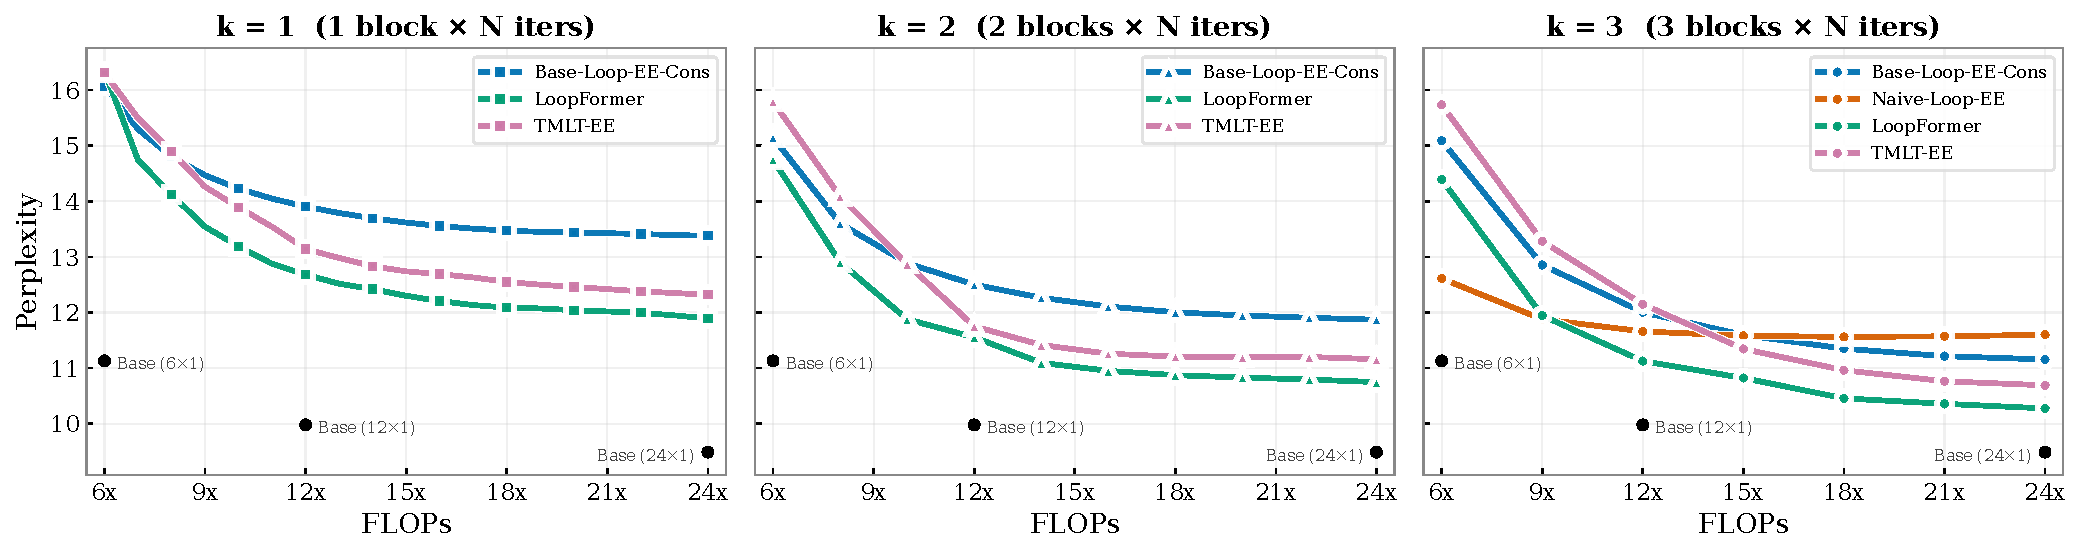
\includegraphics[width=\linewidth]{assets/perplexity_by_k.pdf}
    

\vspace{-4mm}
    
  \caption{Scaling with layers and loops.
    Perplexity on The Pile across $(k,L)$ and inference budgets $M\le L$; larger $k$ lowers perplexity at fixed $M$, and additional loops further reduce it.}

\label{fig:perplexity_graph}
\end{figure*}


\begin{figure*}[t]
  \centering

    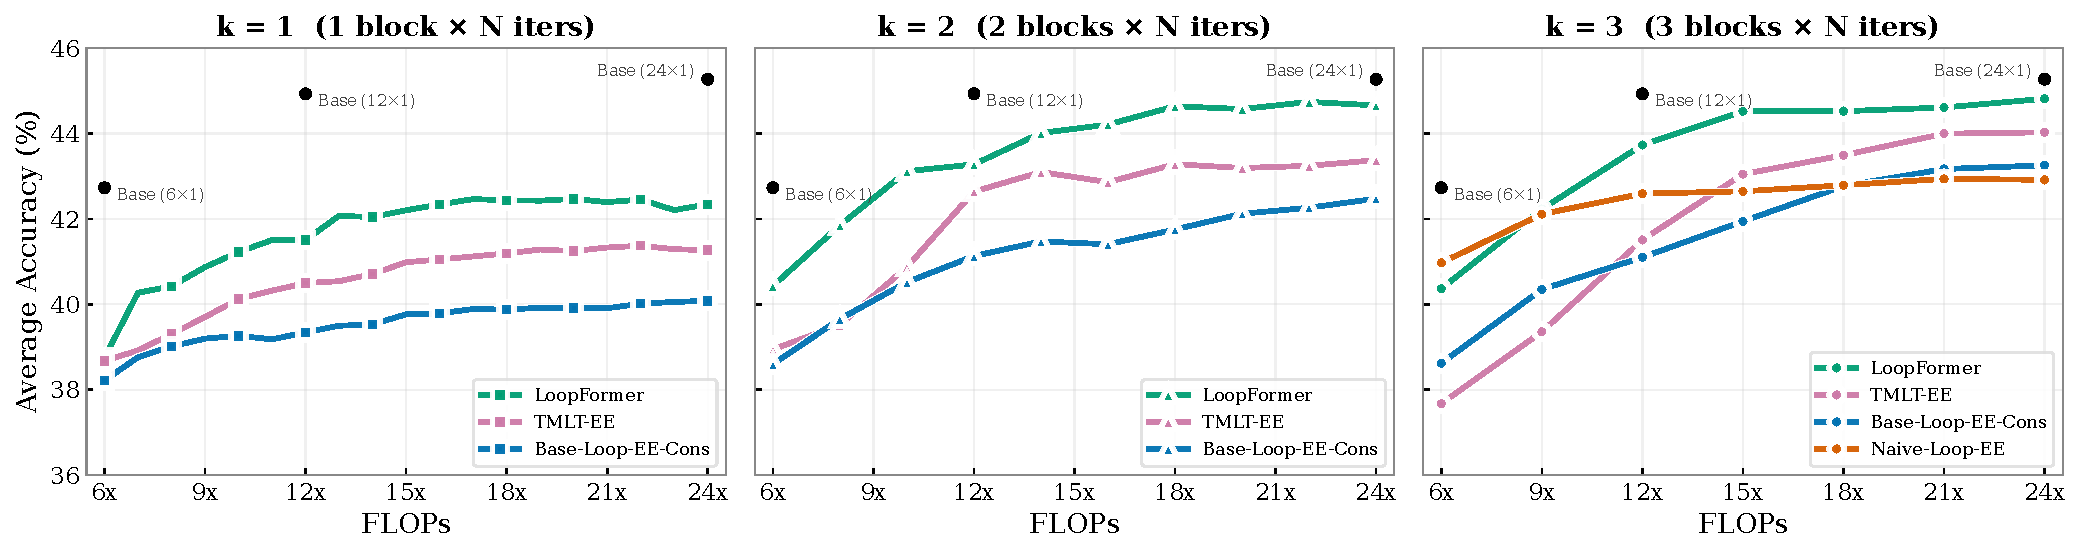
\includegraphics[width=\linewidth]{assets/reasoning_by_k.pdf}
    

    \vspace{-4mm}
    
  \caption{Scaling with layers and loops.
    Average zero-shot reasoning accuracy on 10 tasks for the same settings; more loops improve reasoning at fixed $k$.
    Across budgets, LoopFormer scales smoothly without collapse and consistently outperforms other looped baselines.}
\label{fig:reasoning_graph}
\end{figure*}








% \vspace{-5mm}
\subsection{Number of Layers vs.\ Number of Loops}
We study how perplexity and reasoning change as the number of Transformer layers per block ($k$) varies. We train $k\in\{1,2,3\}$ with maximum loops $L\in\{8,12,24\}$, then evaluate across multiple inference budgets ($M\le L$). \autoref{fig:perplexity_graph} reports perplexity and \autoref{fig:reasoning_graph} reports average zero-shot reasoning accuracy across benchmarks.


% As the plots show, both perplexity and reasoning improve with larger $k$ and more iterations. Crucially, LoopFormer preserves these trends under budget constraints ($M\le L$): shorter trajectories remain informative and additional loops yield smooth gains without representational collapse. Moreover, our consistency-augmented training improves the scaling behavior of Base-Loop and TMLT in the depth-elastic regime.

As the plots show, both perplexity and reasoning improve with larger $k$ and more iterations. \textbf{LoopFormer} preserves these trends under budgets ($M\le L$): shorter trajectories remain informative and added loops yield smooth gains without collapse. Our consistency-augmented training also improves the scaling of Base-Loop and TMLT in the depth-elastic regime.




\begin{figure*}[t]
  \centering

  % Panels
  \begin{subfigure}[t]{0.32\textwidth}
    \centering
    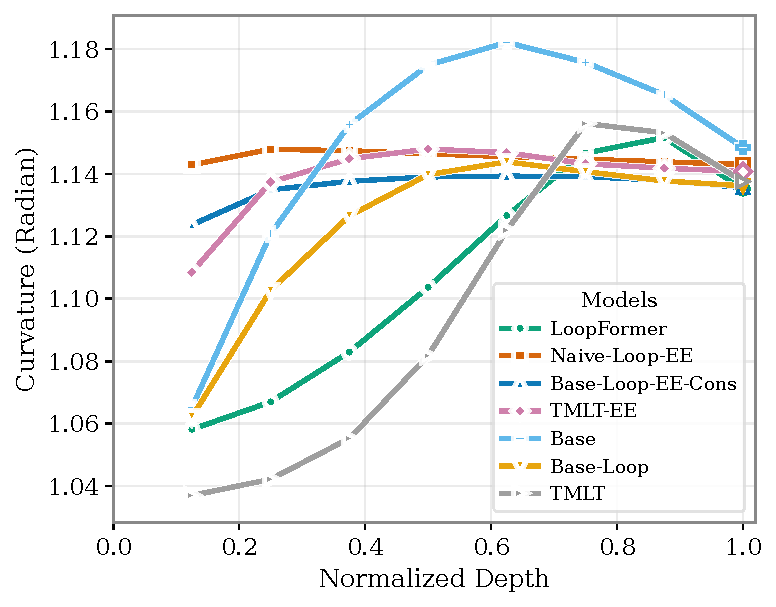
\includegraphics[width=\linewidth]{assets/curvature.pdf}
    \subcaption{Curvature}
    \label{fig:curvature}
  \end{subfigure}
  \hfill
  \begin{subfigure}[t]{0.32\textwidth}
    \centering
    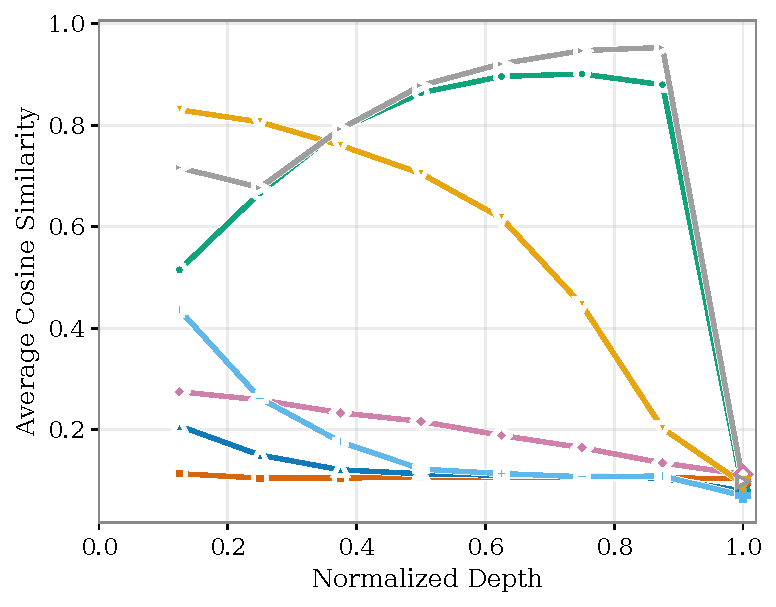
\includegraphics[width=\linewidth]{assets/cosine_distance.pdf}
    \subcaption{Anisotropy}
    \label{fig:anisotropy}
  \end{subfigure}
  \hfill
  \begin{subfigure}[t]{0.32\textwidth}
    \centering
    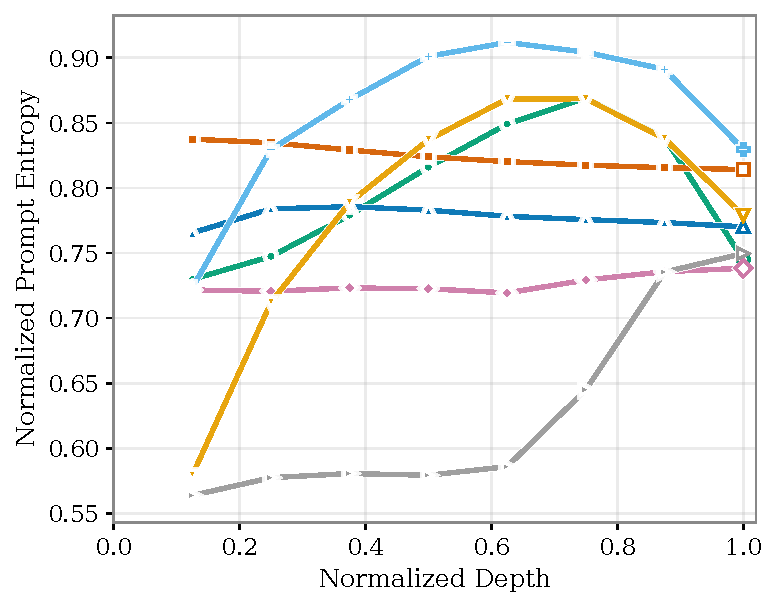
\includegraphics[width=\linewidth]{assets/prompt_entropy.pdf}
    \subcaption{Prompt Entropy}
    \label{fig:prompt_entropy}
  \end{subfigure}

      \caption{Representation metrics over normalized depth. Panels show \textbf{(a)} curvature, \textbf{(b)} anisotropy, and \textbf{(c)} normalized prompt entropy. Early-exit baselines remain flat, indicating minimal change with additional loop steps, whereas LoopFormer exhibits sustained evolution that rises through mid-depths and tapers near the end, suggesting useful depth-elastic dynamics.}

  \label{fig:representation_metrics}
\end{figure*}

\begin{figure*}[t]
  \centering
  \begin{subfigure}[t]{0.32\textwidth}
    \centering
    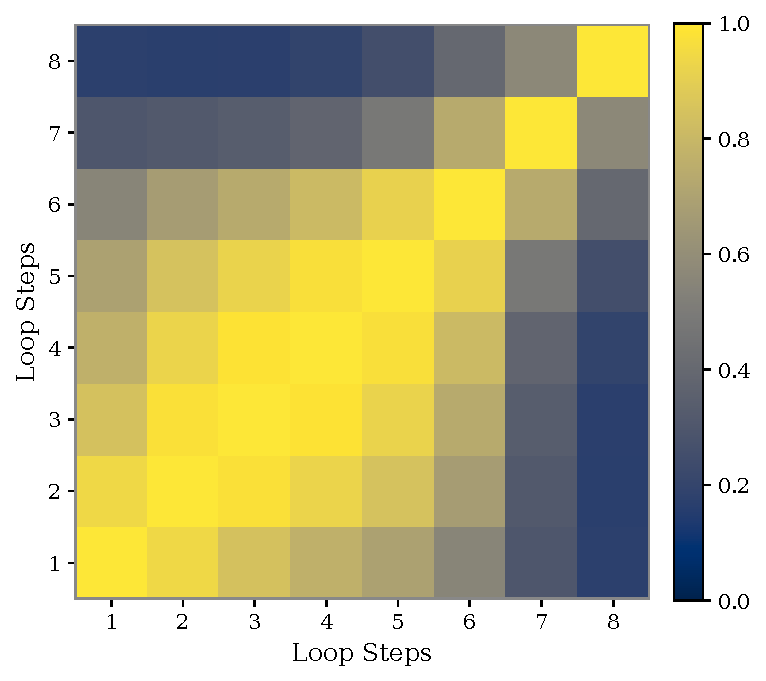
\includegraphics[width=\linewidth]{assets/shortcut_cka.pdf}
    \subcaption{LoopFormer}
    \label{fig:cka_loopformer}
  \end{subfigure}
  \hfill
  \begin{subfigure}[t]{0.32\textwidth}
    \centering
    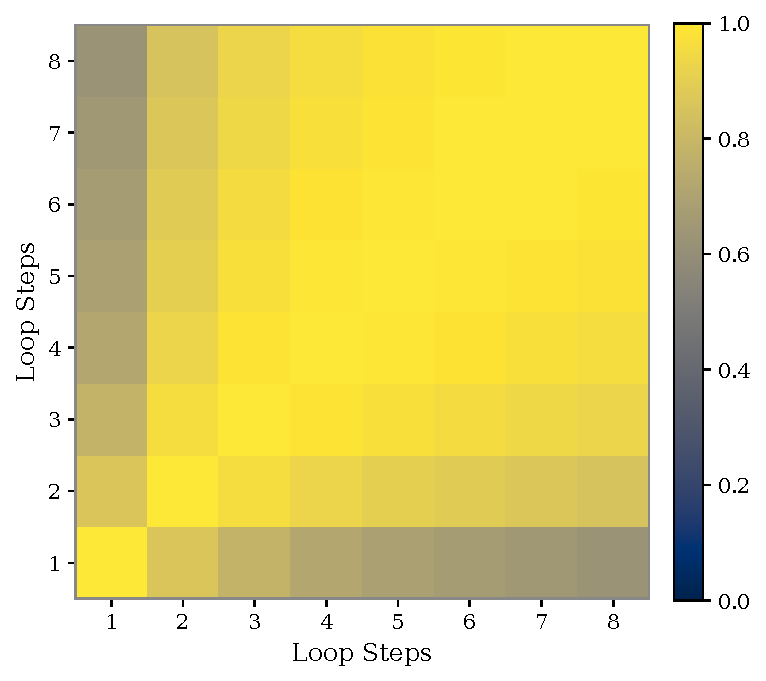
\includegraphics[width=\linewidth]{assets/albert_ee_cka.pdf}
    \subcaption{Base-Loop-EE-Cons}
    \label{fig:cka_base_loop_ee}
  \end{subfigure}
  \hfill
  \begin{subfigure}[t]{0.32\textwidth}
    \centering
    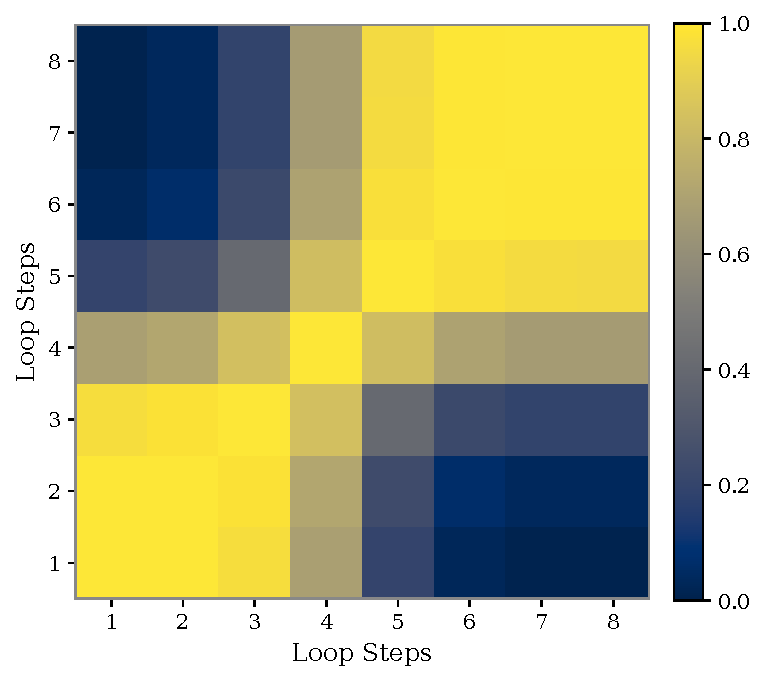
\includegraphics[width=\linewidth]{assets/tmlt_ee_cka.pdf}
    \subcaption{TMLT-EE}
    \label{fig:cka_tmlt_ee}
  \end{subfigure}

  \caption{CKA similarity across loop steps. Each heatmap reports cross-step CKA within a model family. Depth-elastic baselines show high CKA (indicating little change across loops), suggesting stagnation. LoopFormer exhibits progressive drift, especially toward the later steps.}



  \label{fig:cka}
\end{figure*}




\subsection{Analyzing Representation Collapse in Looped Transformers}

The role of depth in Transformers has been widely examined through scaling laws and theory \cite{kaplan2020scaling, csordas2025language}, with a recurring observation that very deep stacks can exhibit \emph{representation degeneration} (or \emph{collapse}), where hidden states change little across layers \cite{ethayarajh2019contextual, dong2021attention, godey2024anisotropy}. Several works attribute this to an inductive bias of self-attention toward uniformity, including rank decay in attention maps with depth \cite{dong2021attention}. Related studies of \emph{anisotropy} \cite{razzhigaev2023shape, godey2024anisotropy} report pronounced effects in language modeling, and these effects could be amplified in looped architectures where a single block is repeatedly applied \cite{dong2021attention}.

We analyze token dynamics along the computation depth using four complementary metrics:
(i) \textbf{anisotropy} \cite{godey2024anisotropy} within a layer, measured as average pairwise cosine similarity among tokens in the prompt; higher values indicate more aligned (less diverse) directions.
(ii) \textbf{Curvature} \cite{hosseini2023large}, a local geometric measure of how rapidly token representations change direction across neighboring positions.
(iii) \textbf{Prompt entropy} \cite{skean2025layer}, a matrix-based estimate of how spread-out token embeddings are across feature dimensions; higher entropy suggests greater diversity and lower redundancy.
(iv) \textbf{CKA similarity} \cite{kornblith2019similarity} across loop steps, quantifying representational similarity between different iterations of the shared block.
While prior work studies these metrics in various architectures and their correlation with downstream performance \cite{garrido2023rankme, skean2025layer}, here we use them primarily as diagnostics to assess whether looped models \emph{use} additional computation (iterative depth) or \emph{stagnate}.

\autoref{fig:representation_metrics} summarizes curvature, anisotropy, and prompt entropy across loop steps; \autoref{fig:cka} reports cross-step CKA. Early-exit looped baselines show flat trajectories on all three metrics and high CKA, indicating stagnation. In contrast, LoopFormer evolves: early steps have lower curvature, weaker angular alignment, and lower entropy; as steps progress, curvature and entropy rise and alignment increases, then all three taper near the final step as the model prepares for unembedding.


Overall, these patterns suggest that LoopFormer maintains \emph{useful} representational dynamics across loops, with shorter trajectories remaining informative and longer trajectories providing additional refinement, rather than converging prematurely to a static state. We view this as evidence that shortcut conditioning and consistency training help avert collapse in depth-elastic looped models. 



\subsection{How to choose trajectories under a fixed budget}

\begin{figure*}[t]
  \centering
  \begin{subfigure}[t]{0.32\textwidth}
    \centering
    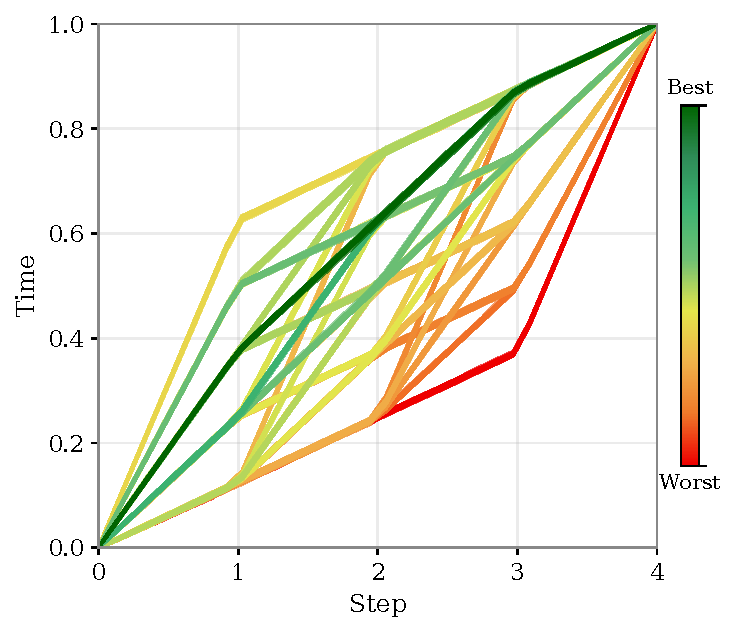
\includegraphics[width=\linewidth]{assets/shortcut_3_ppl.pdf}
    \subcaption{Perplexity ($3 \otimes 8$; $M=4$)}
    \label{fig:space_ppl_3_8}
  \end{subfigure}
  \hfill
  \begin{subfigure}[t]{0.32\textwidth}
    \centering
    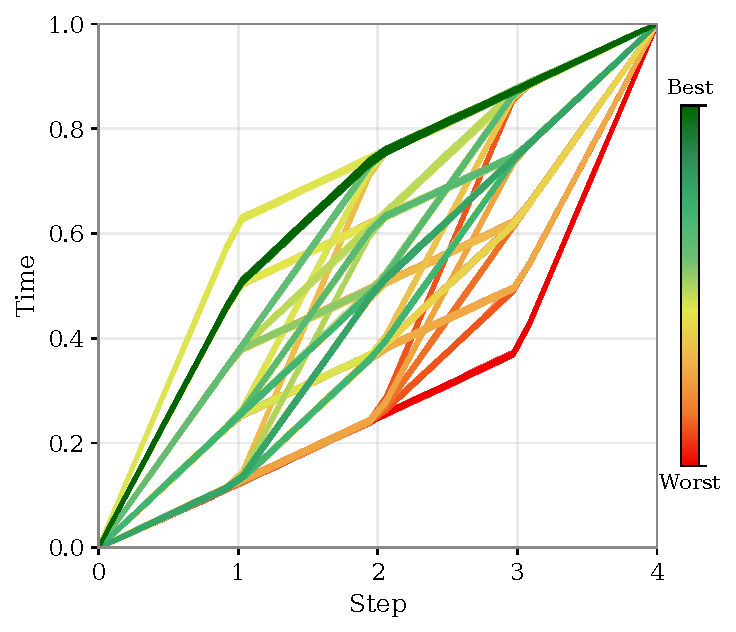
\includegraphics[width=\linewidth]{assets/shortcut_3_acc.pdf}
    \subcaption{Accuracy ($3 \otimes 8$; $M=4$)}
    \label{fig:space_acc_3_8}
  \end{subfigure}
  \hfill
  \begin{subfigure}[t]{0.32\textwidth}
    \centering
    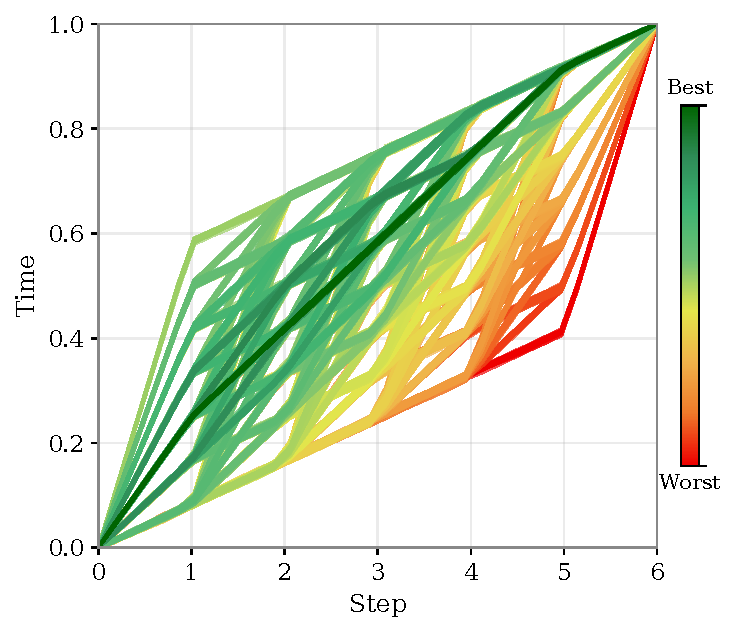
\includegraphics[width=\linewidth]{assets/shortcut_2_ppl.pdf}
    \subcaption{Perplexity ($2 \otimes 12$; $M=6$)}
    \label{fig:space_ppl_2_12}
  \end{subfigure}

  \caption{Performance across length-$M$ trajectories. \textbf{(a,b)} enumerate all $M{=}4$ schedules for LoopFormer $(3\otimes 8)$, reporting perplexity and average zero-shot accuracy; \textbf{(c)} shows perplexity for $M{=}6$ schedules of $(2\otimes 12)$. Even at fixed budget, trajectory choice matters: spreads are large, and top schedules allocate coarser steps early and finer steps late.}
  \label{fig:time_space}
\end{figure*}

A practical question for our depth-elastic models is: \emph{given a budget $M\le L$, how should we choose $\boldsymbol{\Delta}_M$?} Beyond average gains, we ask which \emph{trajectories} work best and which parts of time contribute most. The representation analyses in \autoref{fig:representation_metrics} and \autoref{fig:cka} suggest a pattern: early steps produce more similar states, activity rises mid/late, then tapers near the end.

% To probe this directly, we run a toy but exhaustive study. For LoopFormer $(3\otimes8)$ with budget $M=4$, we enumerate all trajectories whose step sizes sum to 1 (aligned to the training granularity), and measure both perplexity and average zero-shot accuracy (\autoref{fig:space_ppl_3_8}, \autoref{fig:space_acc_3_8}). Despite identical compute, performance varies notably across schedules (spread $\sim$1.4 PPL and $\sim$1.3 accuracy points). We repeat for $(2\otimes12)$ with $M=6$, which yields many more trajectories; the perplexity spread is larger (nearly 3; \autoref{fig:space_ppl_2_12}).

To probe this directly, we run a toy yet exhaustive study. For LoopFormer $(3\otimes8)$ with budget $M=4$, we enumerate all trajectories with step sizes summing to 1 (aligned to training granularity) and measure perplexity and average zero-shot accuracy (\autoref{fig:space_ppl_3_8}, \autoref{fig:space_acc_3_8}). Despite identical compute, performance varies across schedules (spread $\sim$1.4 perplexity and $\sim$1.3 accuracy points). Repeating for $(2\otimes12)$ with $M=6$, the perplexity spread grows to nearly 3 (\autoref{fig:space_ppl_2_12}).


\paragraph{Findings.}
(1) Even under uniform training over budgets and times, some schedules outperform others by wide margins.  
(2) The best schedules for perplexity and for downstream reasoning are close but not identical; both favor allocating larger steps early and finer steps late.